\documentclass{article}
\pagestyle{empty}
\usepackage{amsmath,amssymb,amsfonts}
\usepackage{graphicx}
\usepackage{multicol}
\setlength{\oddsidemargin}{0in} \setlength{\evensidemargin}{0in}
\setlength{\topmargin}{0in} \setlength{\textheight}{8.5in}
\setlength{\textwidth}{6.5in}

\begin{document}
\begin{flushleft}
	\bfseries{MATH 260, Linear Systems and Matrices, Fall `14}\\
	\bfseries{Activity 1:  Linear equations and systems, geometrically}\\
	%\bfseries{Honor Code:} \hspace{3.5in}\bfseries{Names:}\\
\end{flushleft}
\begin{flushleft}
\vspace{.25in}

In previous courses you learned about lines and plotting. Today we'll be reviewing a lot of that as a precursor to a more holistic view of systems and LINEar algebra.

\section*{Problem 1:  Plotting 2 variables}
\vspace{0.1in}

a) The point-slope form of a line is $y=mx+b$. This is generally easily graphed, most of our equations though will take `standard' form of: $a_1 x + a_2 y = b$. For practice plot the following line below: $3y-6x=6$.


\newpage

b) Now sketch the following pairs of equations, each pair on its own set of axes:\\
(i) $y=3+2x$ and $y=2x-4$\\
(ii) $3x+7=y$ and $y=\frac{-2}{3}x-1$\\
(iii) $y=2x+1$ and $3y-3=6x$

\vspace{4in}

c) When we plot lines, the intersection gives a pair of $(x,y)$ values which will satisfy both equations. How many such pairs do each of the above sets of lines have?\\

\vspace{1in}

Can you draw a pair of lines which has exactly TWO solutions? Can you come up with any other counts for solutions besides those depicted above?

\newpage
d) Now plot the pair of lines from (b-ii) together with a third line each listed below.\\
(i) First, graph $3x+7=y$ and $y=\frac{-2}{3}x-1$ together with $y+1=\frac{-1}{4}x$ \\
(ii) Second (on a new set of axes), graph $3x+7=y$ and $y=\frac{-2}{3}x-1$ together with $y=\frac{5}{11}$\\

\vspace{4in}

Similar to having two equations, 3 equations can produce the same types of solution sets: None, one or infinite. Only two of which you've plotted. Notice that we really only needed two equations to get the interesction for (ii), this is called ``overdetermined." Case (i) would be called ``inconsistent" or ``indeterminite." 

\vspace{0.3in}
\newpage
\section*{Problem 2: Plotting 3 variables}
\vspace{0.1in}
First, actually plotting an equation with 3 variables can be very challenging.  We've shown the result (when the equation is linear) below, which creates a plane.\\

\vspace{0.1in}

\begin{center}
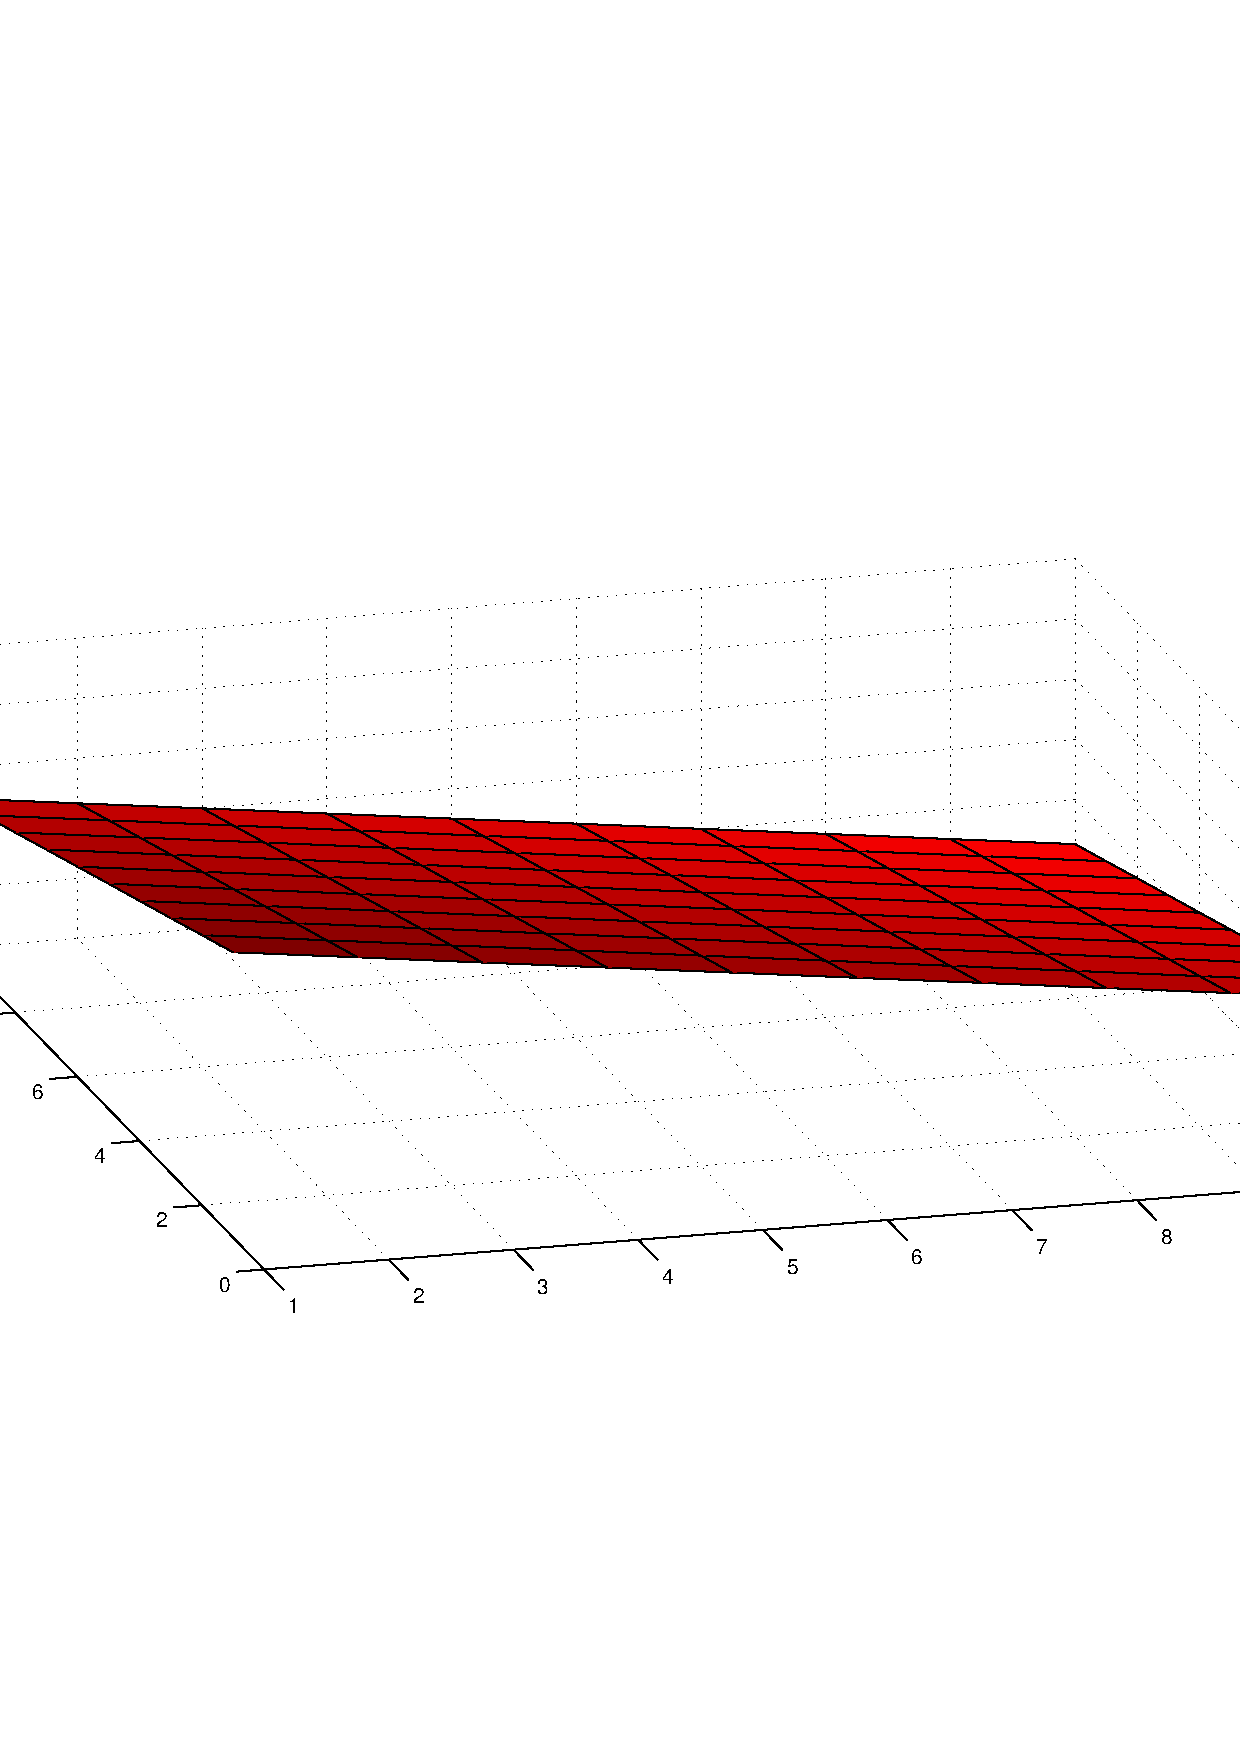
\includegraphics[scale=1.0]{planepic.png}
\end{center}

\vspace{0.1in}

Let's look at another system, this time with 3 variables:\\
$x=3z-2y+1$\\
$3z-2y+x=2$\\
Solve this for $x$, $y$, $z$. \textit{Hint: Solve for $z$ first by substituting the first equation into the second}\\

\vspace{4in}

Did you get numbers for each variable? What do you think is going on here?

\pagebreak

\section*{Problem 3}
Solve the following systems by substitution and/or elimination:

\vspace{0.2in}

a)
\begin{align*}
x+y&=4\\
x-y&=0
\end{align*}
\vspace{0.1in}

\vspace{2in}

b)
\begin{equation*}
\begin{array}{ccccccr}
x& + &2y&+&z&= &4\\
x& - & y& & &= &2\\
2x&- & y&+&2z&=&3\\
  &  &3y&+& z&=&2
\end{array}
\end{equation*}

\end{flushleft}
\end{document}